\documentclass[11pt]{article}

\usepackage[T1]{fontenc}
\usepackage{amsmath,amssymb}
\usepackage{graphicx}
\usepackage{float}
\usepackage{geometry}
\usepackage{booktabs}
\usepackage{enumitem}

\geometry{margin=2.5cm}

\begin{document}

\title{Numerical Section}
\date{}
\maketitle

Temperature and prices can be written as the sum of a deterministic component and a stochastic component. Before studying the stochastic part, we first identify and remove the deterministic component.

\medskip

\section{Deseasonalisation}\label{sec:Deseasonalisation}

For hourly temperature, the deterministic part mainly comes from the daily and yearly cycles. The interaction between these cycles should also be taken into account. For example, the temperature at a given location at 8 AM in December and in August is not the same. In addition, temperature may show a long-term trend over the years. In this paper, we use Fourier series to model the daily and yearly seasonalities and their interaction.

\medskip

For hourly prices, other seasonal effects should be considered in addition to the daily and yearly ones, in particular weekly and monthly seasonality. The seasonal behavior of electricity prices is more complex, and several methods have been proposed in the literature. We use a method proposed by Florentina Paraschiv, which combines a yearly structure based on daily prices and an intraday structure based on hourly prices.


\section{Deseasonalise temperature}
We write the temperature as
\[
y(t)=T(t)+S(t)+\varepsilon(t),
\]
where
\[
\begin{aligned}
T(t)           &\text{ is the trend component},\\
S(t)           &\text{ is the seasonal component},\\
\varepsilon(t) &\text{ is the stochastic component}.
\end{aligned}
\]

We take the trend to be constant:
\[
T(t)=\alpha.
\]

We write the seasonal component as
\[
S(t)=S_1(t)+S_2(t),
\]
where \(S_1\) models the daily and yearly seasonalities, and \(S_2\) models their interaction.

We define
\[
S_1(t)=S_{1,\mathrm{day}}(t)+S_{1,\mathrm{year}}(t),
\]
with
\[
\begin{aligned}
S_{1,\mathrm{day}}(t)
&=
\sum_{k=1}^{3}
\left[
a_{k,\mathrm{day}}\cos\left(\frac{2k\pi t}{24}\right)
+
b_{k,\mathrm{day}}\sin\left(\frac{2k\pi t}{24}\right)
\right],
\\[1.2ex]
S_{1,\mathrm{year}}(t)
&=
\sum_{k=1}^{3}
\left[
a_{k,\mathrm{year}}\cos\left(\frac{2k\pi t}{365.25}\right)
+
b_{k,\mathrm{year}}\sin\left(\frac{2k\pi t}{365.25}\right)
\right].
\end{aligned}
\]

Then we define
\[
\begin{aligned}
S_2(t)
&=
\sum_{i=1}^{3}\sum_{j=1}^{3}
\cos\left(\frac{2i\pi t}{24}\right)
\left[
c_{ij}\cos\left(\frac{2j\pi t}{365.25}\right)
+
d_{ij}\sin\left(\frac{2j\pi t}{365.25}\right)
\right]
\\
&\quad+
\sum_{i=1}^{3}\sum_{j=1}^{3}
\sin\left(\frac{2i\pi t}{24}\right)
\left[
e_{ij}\cos\left(\frac{2j\pi t}{365.25}\right)
+
f_{ij}\sin\left(\frac{2j\pi t}{365.25}\right)
\right].
\end{aligned}
\]

\bigskip

\begin{figure}[H]
\centering
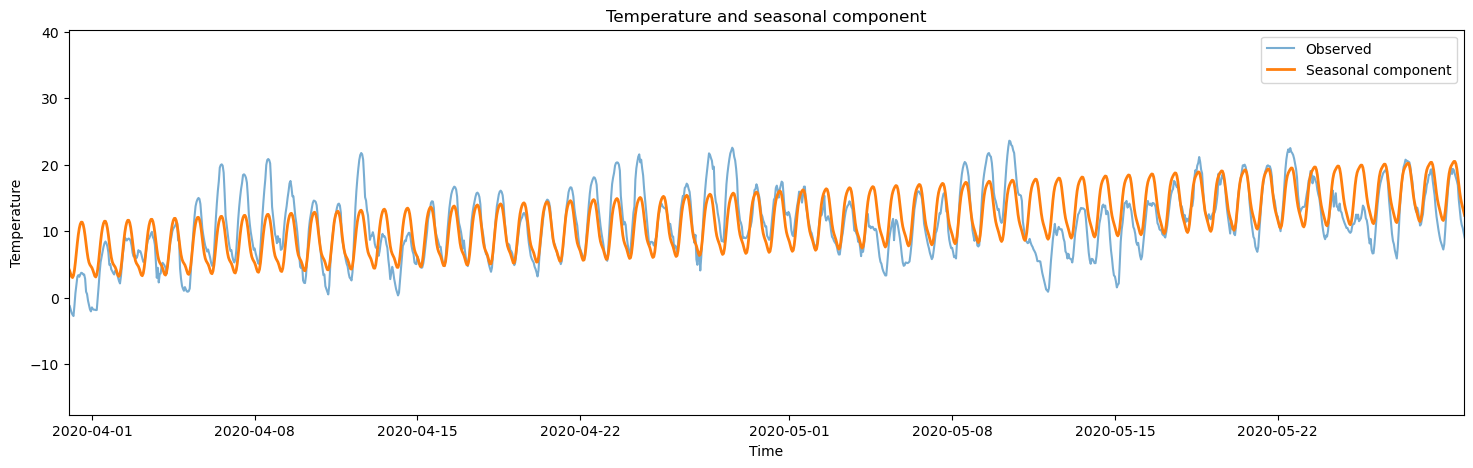
\includegraphics[width=0.95\textwidth]{figure1.png}
\caption{Temperature series and estimated seasonal component.}
\label{fig:temperature_seasonal}
\end{figure}

\begin{figure}[H]
\centering
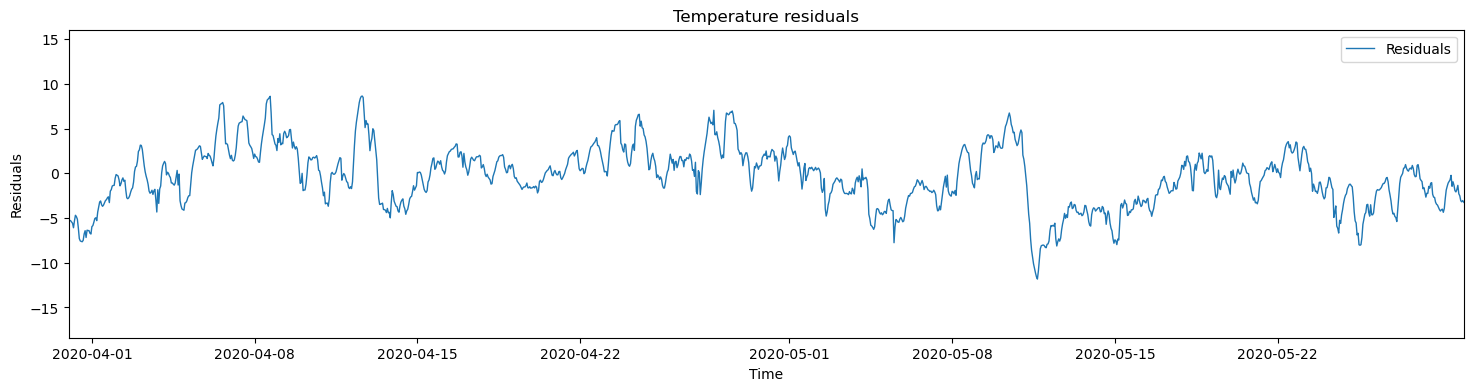
\includegraphics[width=0.95\textwidth]{figure2.png}
\caption{Temperature residuals after deseasonalisation.}
\label{fig:temperature_residuals}
\end{figure}

\begin{figure}[H]
\centering
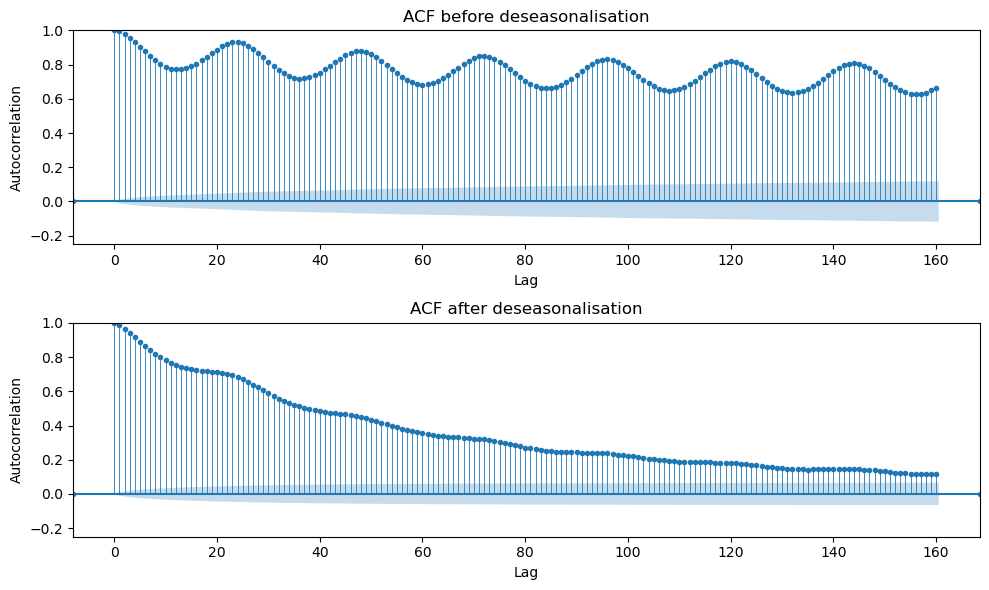
\includegraphics[width=0.85\textwidth]{figure3.png}
\caption{Autocorrelation function before and after deseasonalisation.}
\label{fig:temperature_acf}
\end{figure}

\section{Deseasonalise prices}

To deseasonalise prices, we decompose prices into two patterns: yearly seasonality and daily seasonality. We define two dependent variables, the factor-to-year \(f2y\) and the factor-to-day \(f2d\).

\medskip
The factor-to-year \(f2y\) is the relative weight of an average daily price compared to the annual base of the corresponding year:
\begin{equation}
f2y_d = \frac{S^{day}(d)}{\sum_{k \in year(d)} S^{day}(k)\,\frac{1}{K(d)}}
\end{equation}

where \(S^{day}(d)\) is the daily spot price on day \(d\), defined as the average of hourly electricity prices on that day, and \(K(d)\) denotes the number of days in the year in which \(S^{day}(d)\) is observed.
\medskip

The factor-to-day \(f2d\) is the weight of the price of a particular hour compared to the daily base price:
\begin{equation}
f2d_t = \frac{S^{hour}(t)}{\sum_{k \in day(t)} S^{hour}(k)\,\frac{1}{24}}
\end{equation}

where \(S^{hour}(t)\) is the hourly spot price at time \(t\).

To explain \(f2y\), we use the following multiple regression model:
\begin{equation}
f2y_d = \alpha_0 
+ \sum_{i=1}^{6} b_i D_{di}
+ \sum_{i=1}^{12} c_i M_{di}
+  d \cdot CDD
+  e\cdot HDD
+ \varepsilon
\end{equation}

\begin{itemize}[leftmargin=1.5em]
\item \(f2y_d\): factor-to-year, daily-base-price/yearly-base-price
\item \(D_{di}\): 6 daily dummy variables (for Monday to Saturday)
\item \(M_{di}\): 12 monthly dummy variables (for February to December); August is subdivided into two parts due to summer vacation

\item Cooling Degree Days (CDD) \(= \max(T - 15^\circ C, 0)\)
\item Heating Degree Days (HDD) \(= \max(15^\circ C - T, 0)\)
\end{itemize}

\begin{figure}[H]
\centering
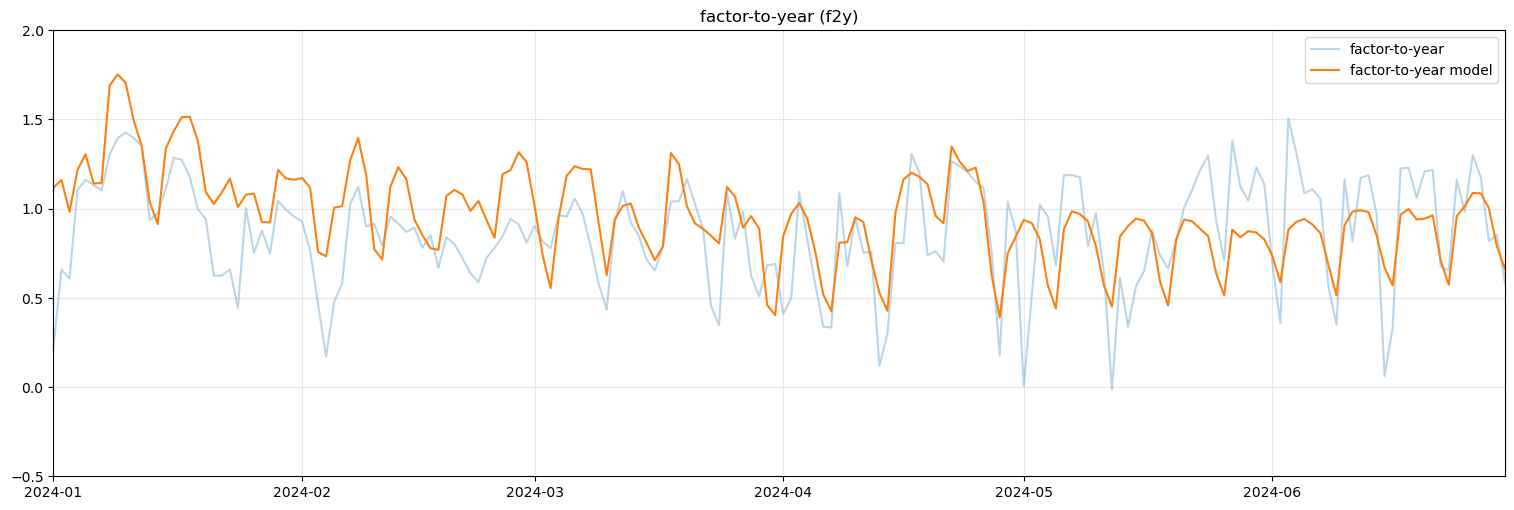
\includegraphics[width=0.90\textwidth]{figure4.png}
\caption{Factor-to-year \((f2y)\) in March 2024.}
\label{fig:f2y_march_2024}
\end{figure}

\bigskip

To explain \(f2d\), we first build different profile classes of days. These classes reflect the fact that prices evolve differently depending on whether the day is a weekday, a Saturday or a Sunday, as well as on the month. Therefore, all workdays within the same month belong to the same profile class, while Saturdays and Sundays are grouped in three-month periods.

\bigskip

\textbf{Table 1.} Assignment of each day to one of the profile classes.

\medskip

\begin{center}
\begin{tabular}{lcccccccccccc}
\toprule
 & J & F & M & A & M & J & J & A & S & O & N & D \\
\midrule
Week day & 1 & 2 & 3 & 4 & 5 & 6 & 7 & 8 & 9 & 10 & 11 & 12 \\
Sat      & 13 & 13 & 14 & 14 & 15 & 15 & 15 & 16 & 16 & 16 & 13 & 13 \\
Sun      & 17 & 17 & 18 & 18 & 19 & 19 & 19 & 20 & 20 & 20 & 17 & 17 \\
\bottomrule
\end{tabular}
\end{center}

\bigskip

For each class, we build the following regression model:
\begin{equation}
f2d_t = a_0^c + \sum_{i=1}^{23} b_i^c H_{t,i} + \varepsilon_t,
\quad \text{for all } t \in c.
\end{equation}

\begin{figure}[H]
\centering
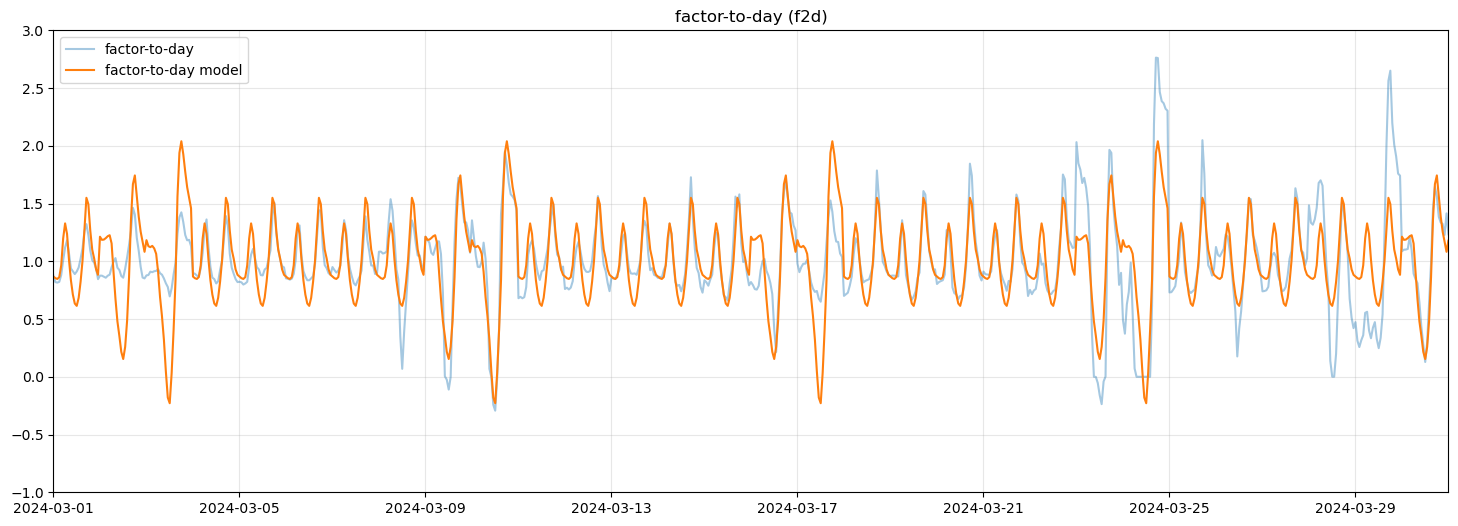
\includegraphics[width=0.95\textwidth]{figure5.png}
\caption{Factor-to-day \((f2d)\) from January to June 2024.}
\label{fig:f2d_jan_jun_2024}
\end{figure}

\bigskip

Finally, the seasonality model \(sw_t\) is defined as the product of \(f2y\) and \(f2d\), multiplied by the average price \(\bar{P}\):
\[
sw_t = f2y_t \cdot f2d_t \cdot \bar{P}.
\]

\begin{figure}[H]
\centering
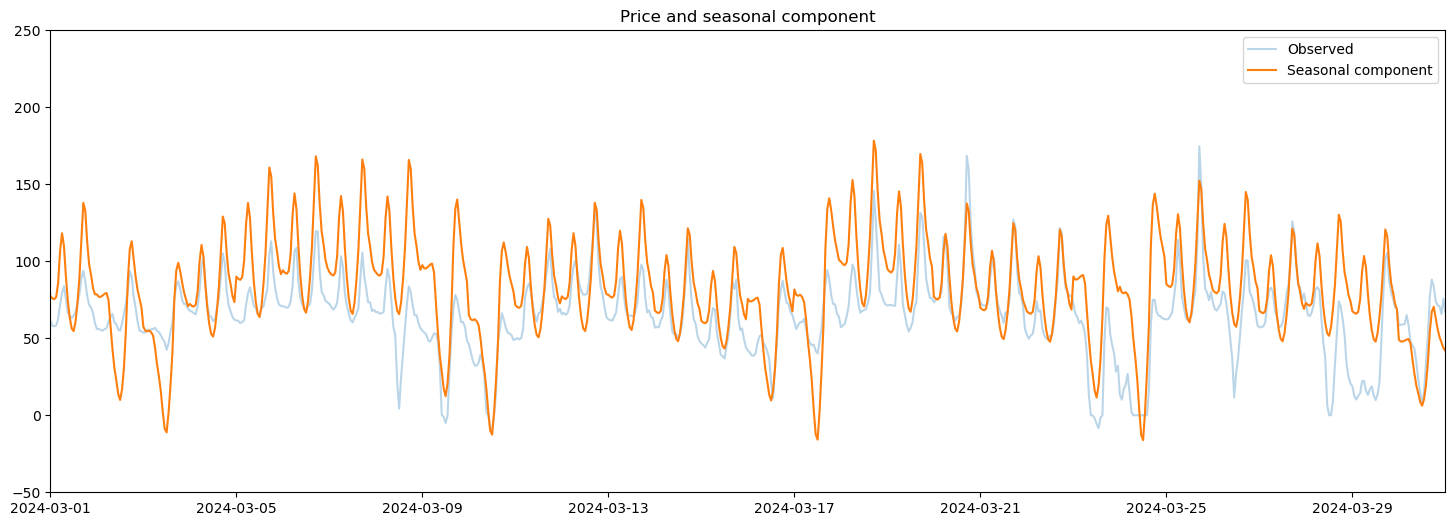
\includegraphics[width=0.95\textwidth]{figure6.png}
\caption{Price series and estimated seasonal component.}
\label{fig:price_seasonal}
\end{figure}

\begin{figure}[H]
\centering
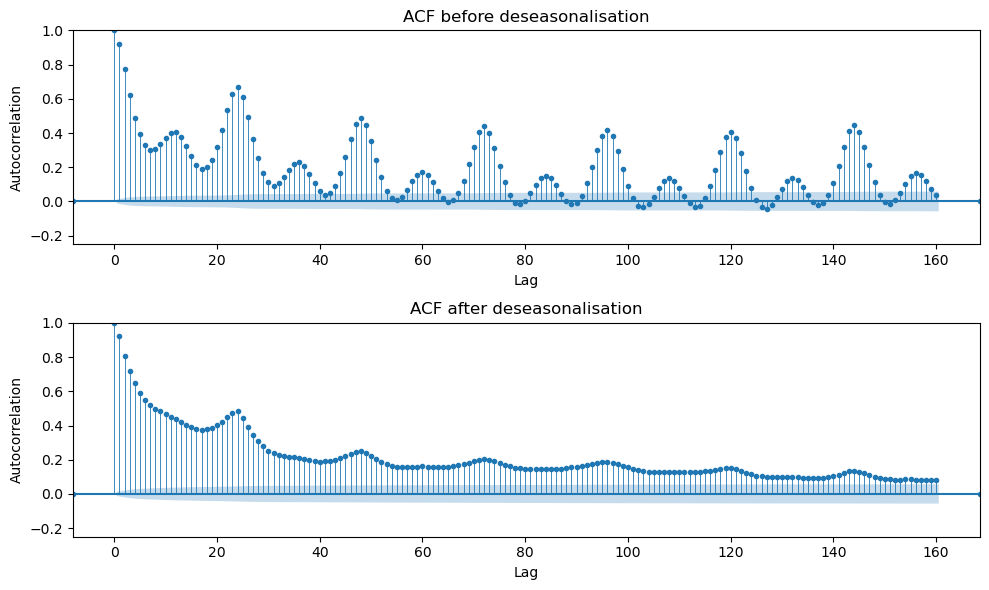
\includegraphics[width=0.85\textwidth]{figure7.png}
\caption{Autocorrelation function before and after deseasonalisation.}
\label{fig:price_acf}
\end{figure}

\end{document}